\subsubsection{Aux clocks}

\begin{figure}[ht]
  \begin{center}
    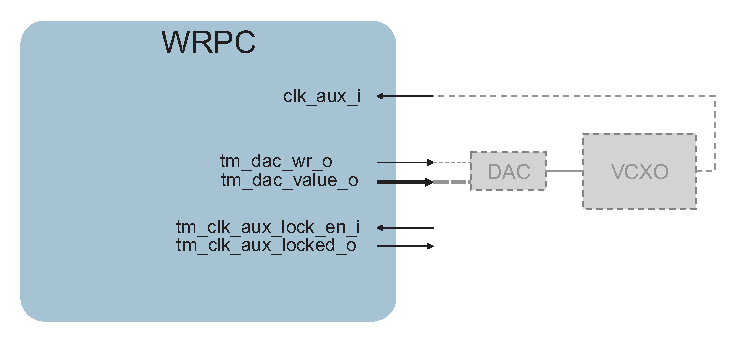
\includegraphics[width=.8\textwidth]{fig/adv_wrpc_clk.pdf}
    \caption{Aux clock synchronization interface}
  \end{center}
\end{figure}

The WRPC can syntonize auxiliary clock signals to the White Rabbit timebase. It
is done with a similar PLL that is used to discipline the local reference clock
(section \ref{basic:clk_rst}). WRPC provides tuning values for the VCXO producing
clock signal which is connected to \emph{clk\_aux\_i}.

\begin{hdlporttable}
\end{hdlporttable}
